\documentclass[10pt]{sig-alternate}
\makeatletter
\def\@copyrightspace{\relax}
\makeatother

\usepackage{hyperref}


\begin{document}

% Copyright
\setcopyright{acmcopyright}

\title{
  % 
\includegraphics[width=0.2\textwidth]{hpi_logo_2017}\\
  \vspace{24pt}
  % In-Memory Trajectory Analysis on Taxi Data
  Comparison of Different Data Layouts for Columnar In-Memory Databases on the Basis of an Application
}
\subtitle{
  Seminar Trends and Concepts 3\\
  Summer Semester 2018
}

\numberofauthors{3}

\author{
  Marcel Jankrift, Sebastian Kliem, Toni Stachewicz\\[12pt]
  Supervisors:\\
  Dr. Matthias Uflacker, Keven Richly
}

\maketitle
\begin{abstract}
The taxi business is an extremely competitive market. Private ridesharing companies such as Uber or Lynx have grown tremendously in the last decade. In order to survive as a traditional taxi company, the drivers have to increase their profit even further. Therefore, we created an application, that analysis taxi data recorded over one day in the city of Shenzhen. We examine which taxis were the most profitable ones by calculating the distances and times driven with a passenger. From this information, we can draw specific recommendations, where to take passengers at a certain time, so that the profit can be maximized.
\end{abstract}

\keywords{Geospatial data, Trajectory analysis, Taxi data, In-Memory}

\section{Motivation}

Traditional taxi companies like to increase their profit. For that, the individual taxi drivers would have to find many passengers and minimize their waiting times. A way to be a  good performing taxi is to stay in a profitable area of the city. For example, where taxi rides are highly needed at a specific time. With our help, the taxi companies can develop new strategies. A simple strategy would be to only accept and assign orders whose destination is in a good area for the expected arrival time. We created an interactive map, which shows the best performing taxis for one day in Shenzhen. This is based on a data set that is explained in section \ref{sec:ds}. The application has some additional information about the taxi density and numbers about pick-ups and drop-offs. Taxi companies could use the application to quickly analyze the collected GPS data.\\

\section{Data Sources}
\label{sec:ds}

The data we used is a freely available collection of GPS information of taxis.\footnote{\href{https://www-users.cs.umn.edu/~tianhe/BIGDATA/UrbanCPS/TaxiData/TaxiData}{https://www-users.cs.umn.edu/$\sim$tianhe/BIGDATA/\\UrbanCPS/TaxiData/TaxiData}} The dataset set has been collected over one day starting at 12 AM and 23:59 PM in the city of Shenzhen, China and the surrounding area. The data does not only contain the GPS location at a certain time, but also the current speed and the taxi's occupancy. The status of a driving taxi has been recorded in an average interval of 26.85 seconds or every 15 seconds in median. In total there are 14,728 trajectories traced resulting in almost 47 million records. The data comes in CSV-format which can be loaded into the SAP HANA database immediately. The total memory consumption without any further optimization (e.g. indices) of the Shenzhen data takes 541 MB.

\subsection{Data Cleansing}
Before we started analyzing the trajectories we had a closer look at the dataset itself. We noticed rather soon, that there are some inconsistencies within data. Hence, we perform data cleansing. In the following paragraphs, we describe our criteria for data cleansing in detail.

\subsubsection{Duplicates}
The data was already imported into the database by our supervisor, when we started our project. Since, we did not want to change the the original data we created an own table. Once we wanted to create a primary key, the database has thrown an error stating that the data has duplicate values. In fact, there are 381 data points occuring not only twice, but also multiple times. We deleted those entries, because they do not add any value to the data and prevent the creation of a primary key.

\subsubsection{Bounding box}
Generally, GPS coordinates are not completely accurate. However, there are points in the data set, that do not make sense, are not even possible or do not fit into the geospatial system of longitudes and latidues. The graphic \ref{fig:bbox} below shows the trajectory with id $22,360$ which passes through the ocean. In order to eliminate such outliers, we use a bounding box (rectangle highlighted in red color). To avoid deleting points that are outside this area, because there a taxi really drove there, we have chosen the rectangle intentionally large. This data cleansing step effects almost 8,000 GPS points.

\begin{figure}[ht]
\centering
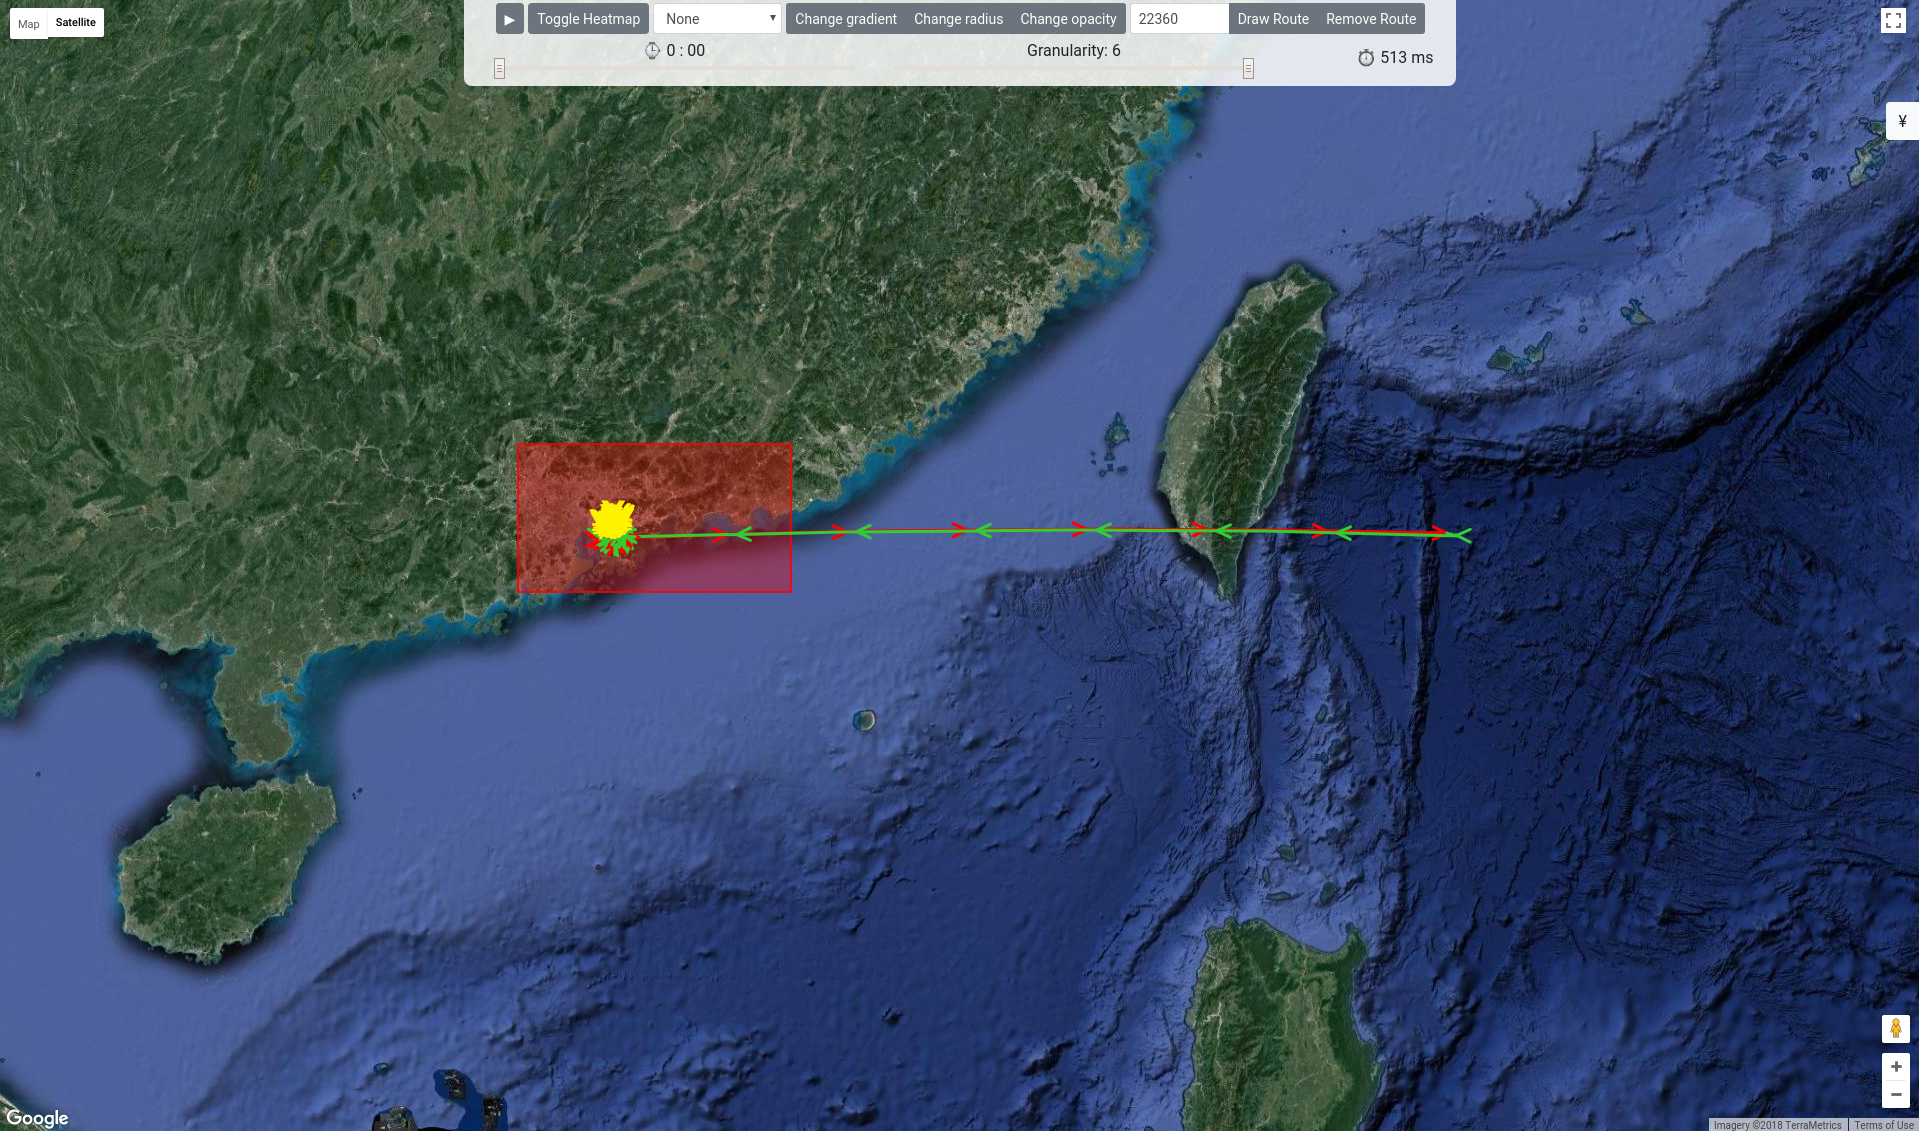
\includegraphics[width=0.5\textwidth]{img/bounding_box.png}
\caption{Bounding box and trajectory $22,360$ passing through the ocean}
\label{fig:bbox}
\end{figure}


\subsubsection{Small trajectories}
\subsubsection{Wrong passenger status}
The status flag indicating the presence of a passenger seems to be wrong in different trajectories. We found three different scenarios and removed the whole trajetory if at least one is fulfilled. First, there are trips passing through the whole city without any passengers at all. Second, the opposite is the case: Taxis do have the same passenger for almost a day. We filtered those trajectories out by adding rules. We assume, that a taxi is supposed to have a passenger for at least two hours (not necessarily continously) and no passenger for at least one hour (also not continously) within the recorded day. In the third case, the passenger status keeps switching over time as depicted in graphic \ref{fig:passenger_status}. In order to avoid wrong calculations based on the false data, we deleted the whole trajectories.


\begin{figure}[ht]
\centering
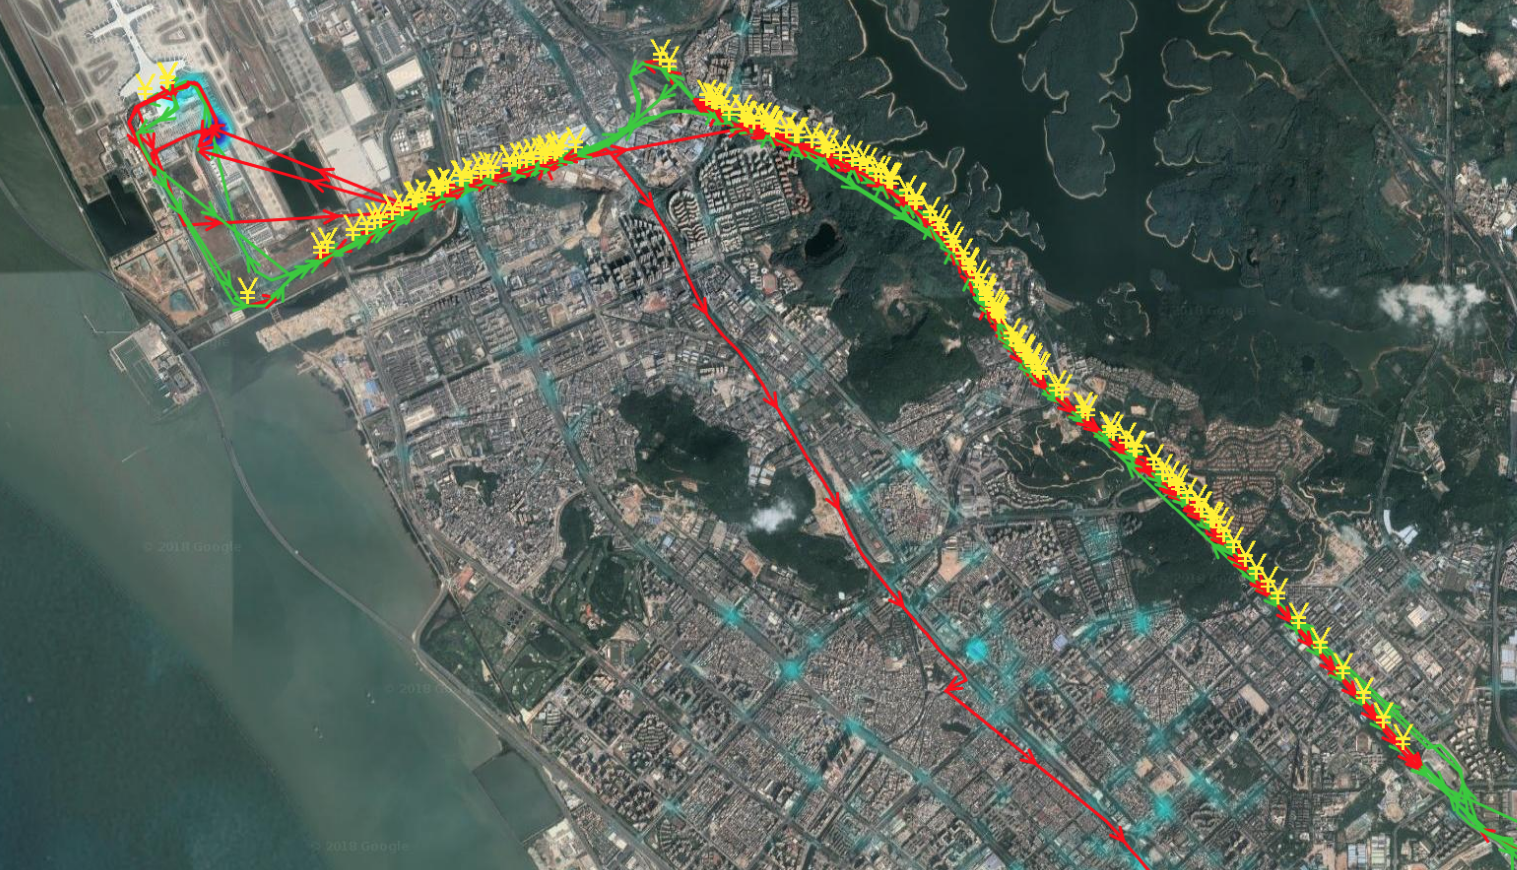
\includegraphics[width=0.5\textwidth]{img/passenger_status.png}
\caption{$27,224$}
\label{fig:passenger_status}
\end{figure}


\subsubsection{Jumps}
GPS data tends to be imprecise by nature. 
\subsubsection{Summary: Data cleansing}

\section{Application Prototype}

The main purpose of our application prototype is to display good performing taxis on a map. Thereby, the user can analyze how taxis get new passengers quickly. An additional task is to visualize the state at a certain time of the day. For that, we created some heatmaps (see section \ref{sec:heatmaps}).

\subsection{Explore Profitable Taxis}

The user can see a ranking of the taxis, which had the most profit during the day. This is shown in figure \ref{fig:ranking}. The list has information about the number of tours. We also calculated the distance of each taxi while passengers were inside. This is displayed in the column \textbf{Distance km}. The profit can be estimated pretty accurately with the help of the distances and the tours' start and end times. We mention distance and profit calculations in section \ref{todo} in more detail. The list is sorted by the estimated profit. It is displayed as the Chinese currency Yuan. When the user clicks on an entry the route for the taxi is drawn on the map.\\

\begin{figure}[ht]
\centering
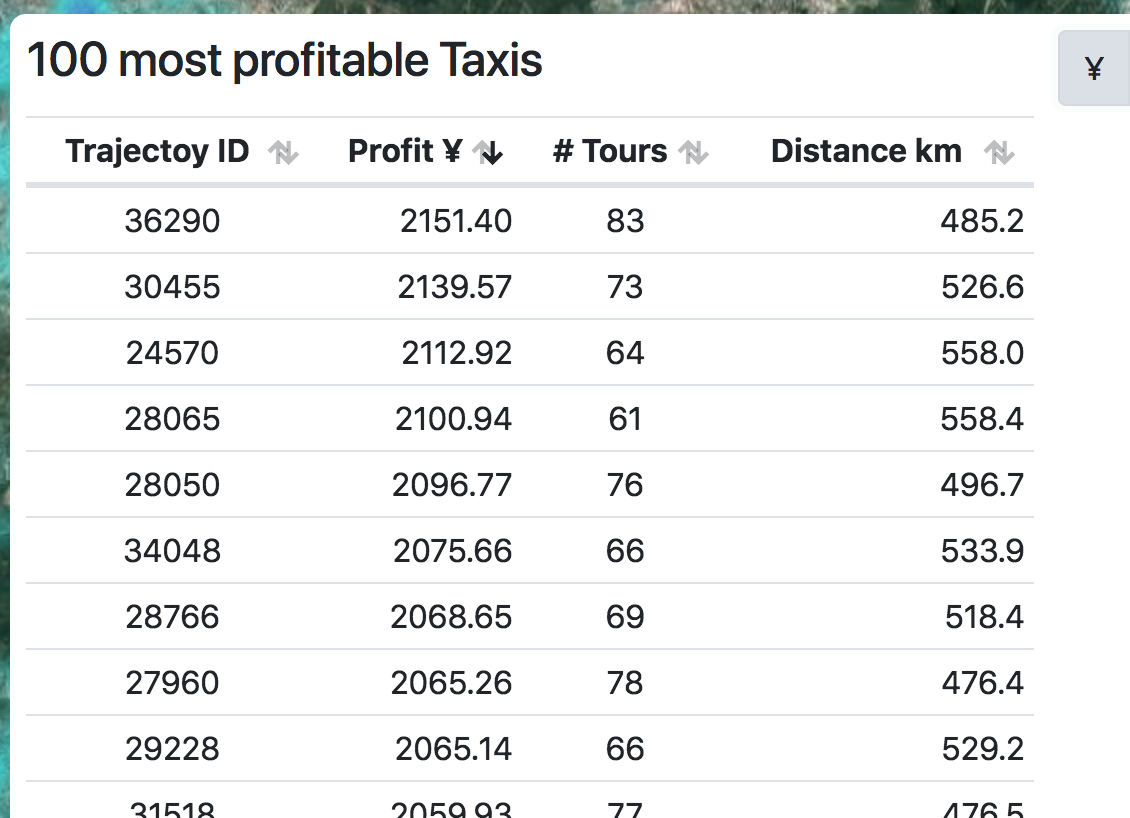
\includegraphics[width=0.5\textwidth]{img/ranking.png}
\caption{Ranking of the most profitable taxis}
\label{fig:ranking}
\end{figure}

Figure \ref{fig:single_ride} illustrates how the taxi routes are drawn. The line is red if the taxi was driven without a passenger. The line is green if it had a passenger. Arrows indicate the direction. At the end of each tour is a a Yuan symbol on which the user can click. The click lets pop up information about the tour (i.e. start time, end time, distance and the estimated profit).\\

\begin{figure}[ht]
\centering
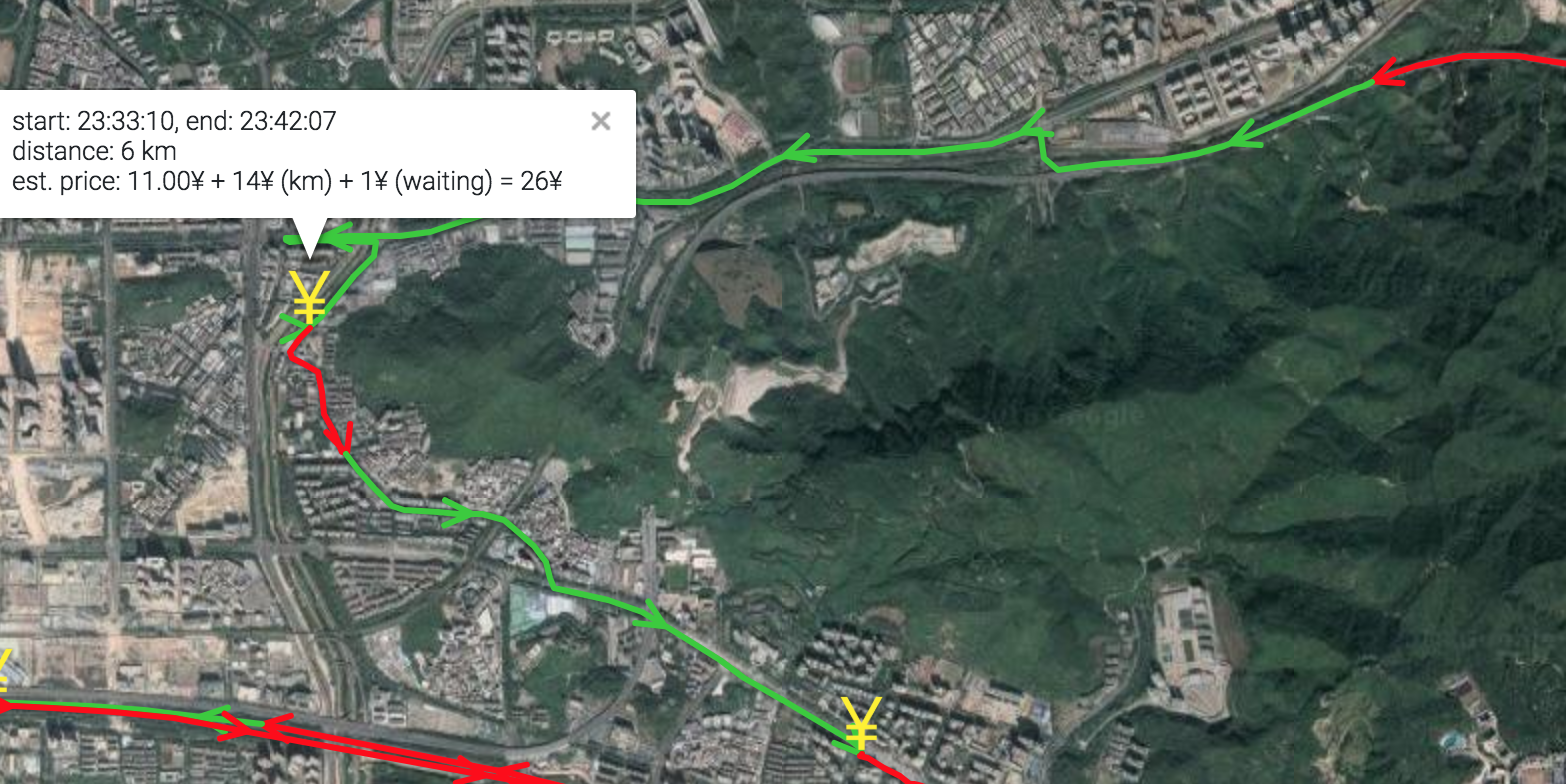
\includegraphics[width=0.5\textwidth]{img/single_ride.png}
\caption{Information about one ride}
\label{fig:single_ride}
\end{figure}

Figure \ref{fig:best_taxi} shows the route of the most profitable taxi (ID \textit{36290} in figure \ref{fig:ranking}). You can see that this taxi had the most tours in one area. The taxi had 83 tours during the day. These tours sum up to a distance of 482 kilometers. The red lines are often very short.

\begin{figure}[ht]
\centering
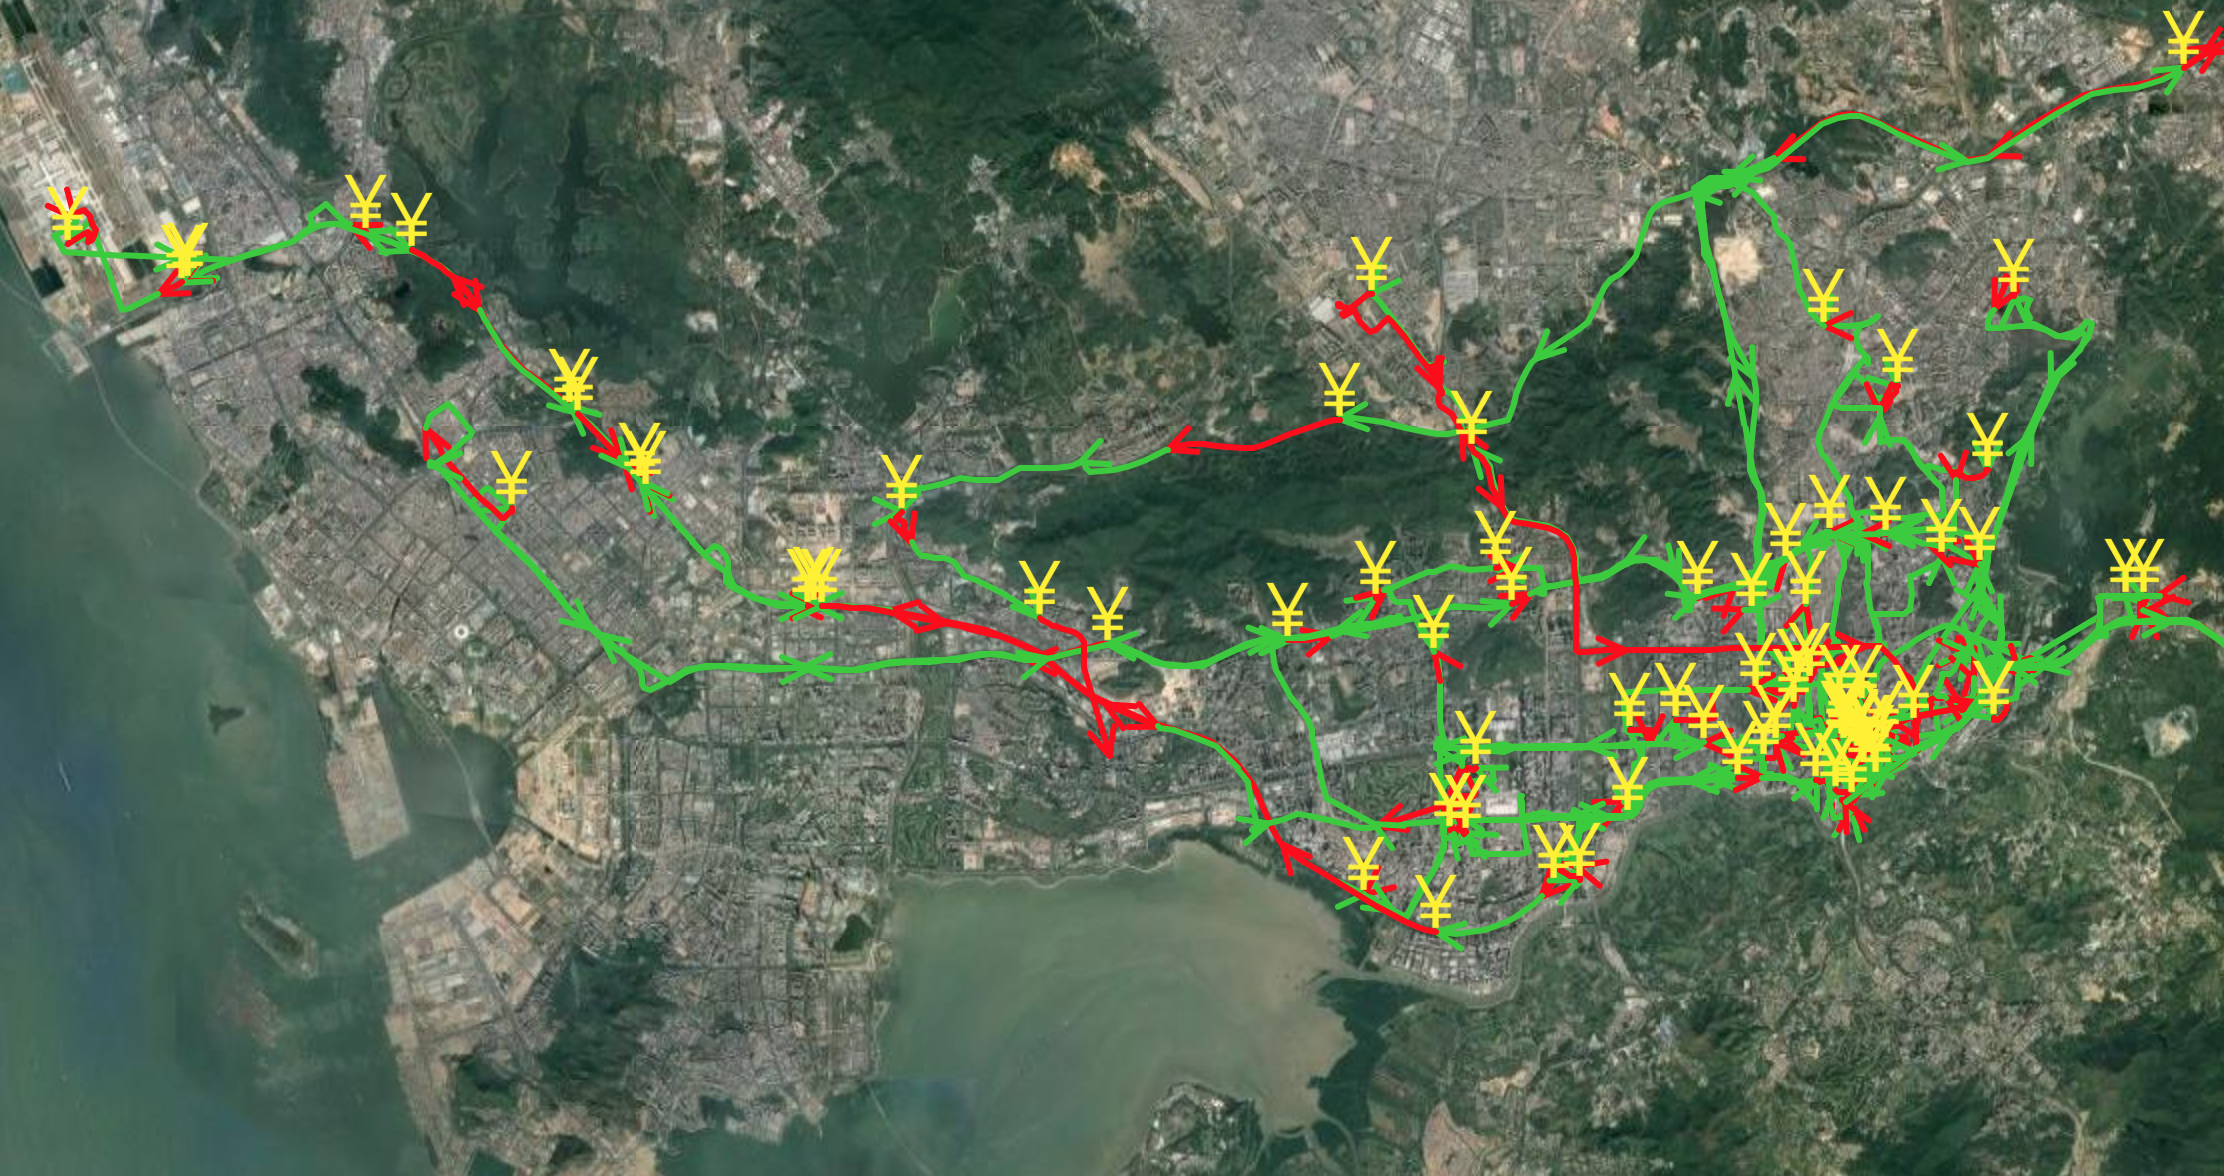
\includegraphics[width=0.5\textwidth]{img/best_taxi.png}
\caption{Entire taxi route}
\label{fig:best_taxi}
\end{figure}

\subsection{Heatmaps}
\label{sec:heatmaps}

The application has a taxi density heatmap (see figure \ref{fig:density}). The areas, which have many taxis at the given time, are colored red. Areas with less taxis are colored blue. The user interface has a time slider. When changing the time from \textit{15:00} to another time, the map would refresh. In the top left corner is a play button. With the play function, the map continually updates to the next time interval. Thus, the user can observe how the taxi density changes over time.

\begin{figure}[ht]
\centering
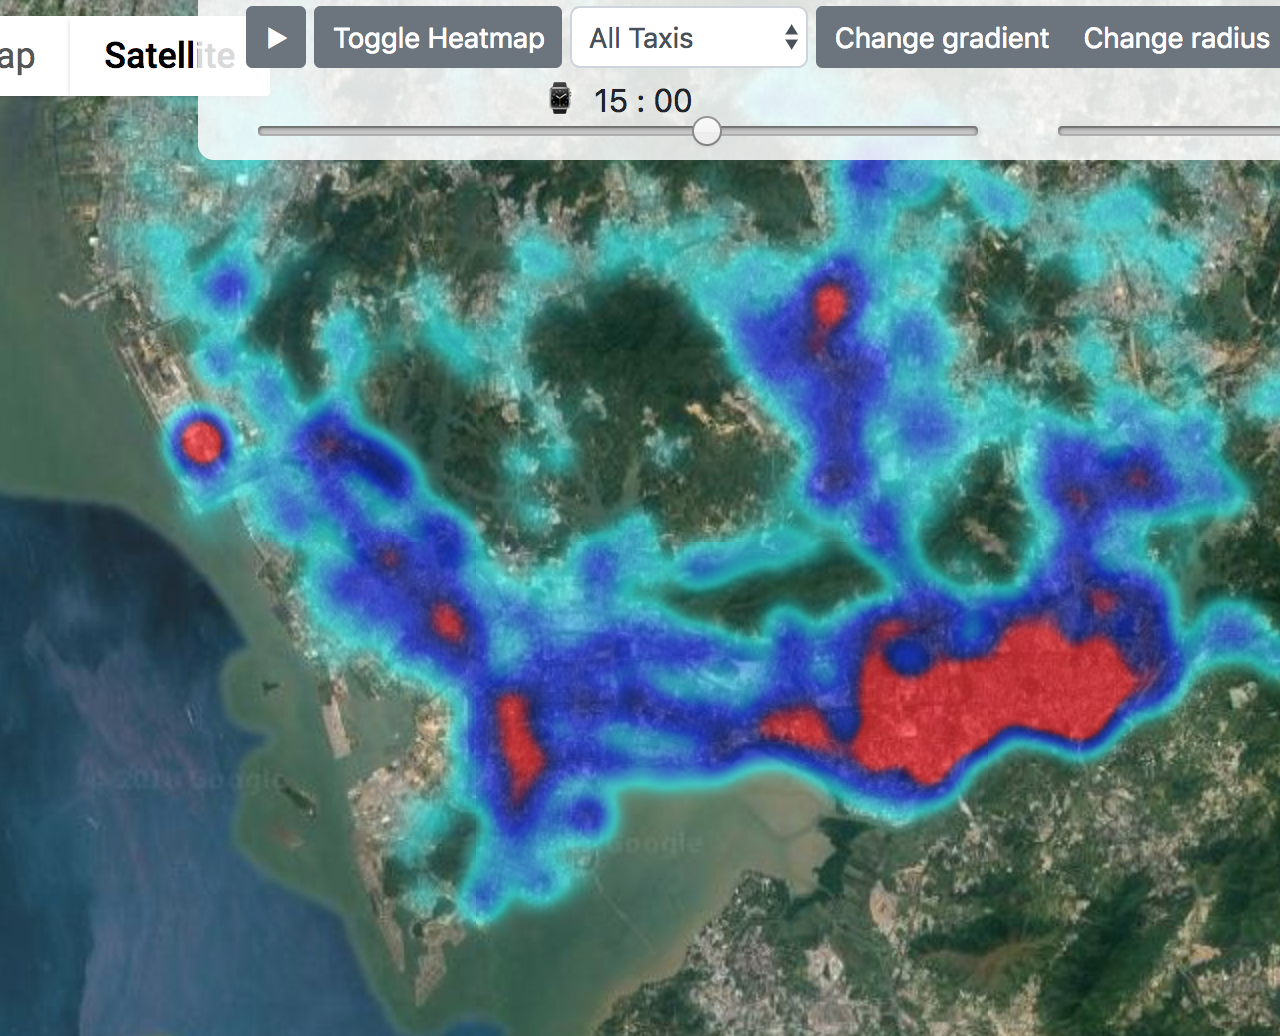
\includegraphics[width=0.5\textwidth]{img/density.png}
\caption{Taxi density heatmap}
\label{fig:density}
\end{figure}

The heatmap can visualize two different things. One of these is the number of picked up passengers. The other one is the number of dropped passengers. Figure \ref{fig:pickup} shows a screenshot with the pickup points heatmap. The user interface has a dropdown menu to let the user select which heatmap is displayed.

\begin{figure}[ht]
\centering
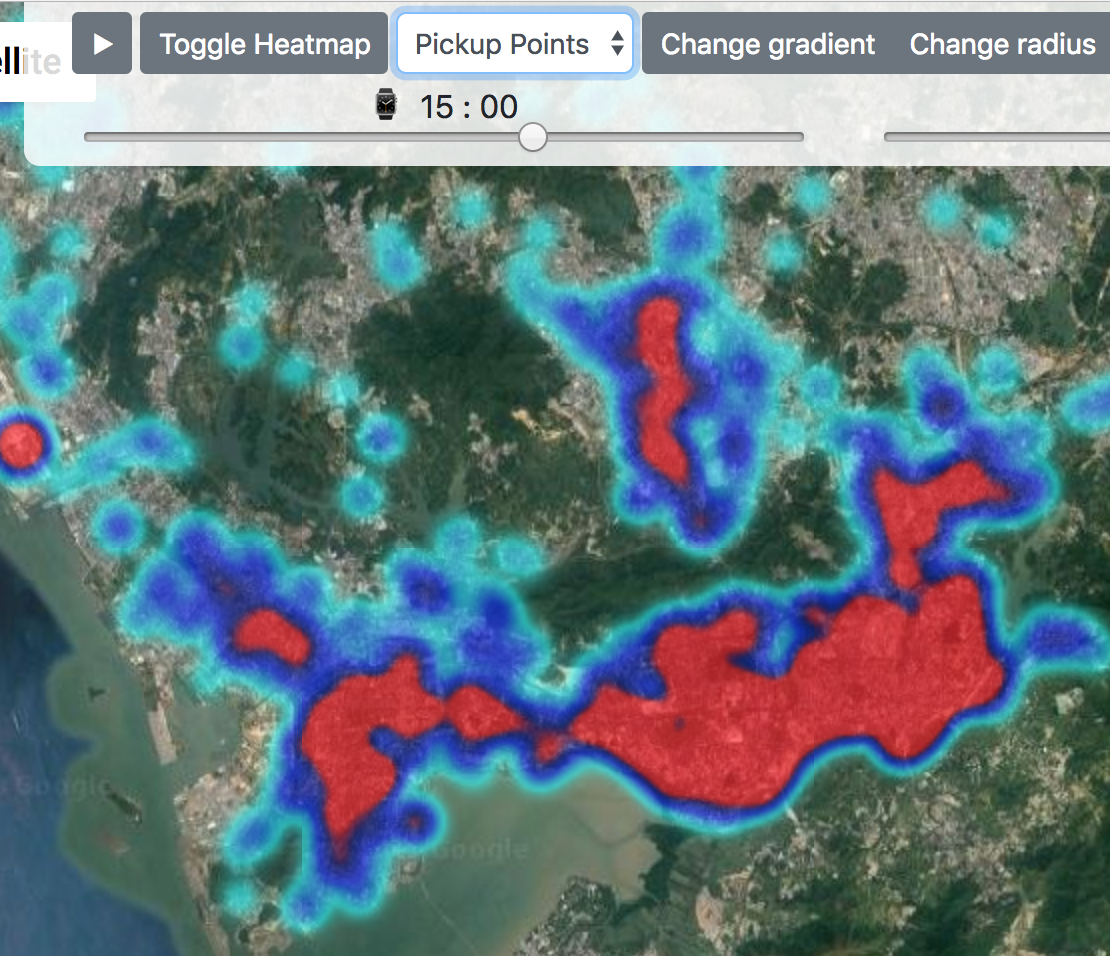
\includegraphics[width=0.5\textwidth]{img/pickup.png}
\caption{Pickup points heatmap}
\label{fig:pickup}
\end{figure}

\subsection{System Architecture}

This section is about our architecture. Figure \ref{fig:architecture} is a FMC (Fundamental Modeling Concepts) diagram. Our architecture can be divided into the three components frontend, backend and database. We have a web application. Hence, it runs in a browser. We are using the Google Maps API. In our frontend, we are using HTML5 and Javascript.\\

\begin{figure*}
\centering
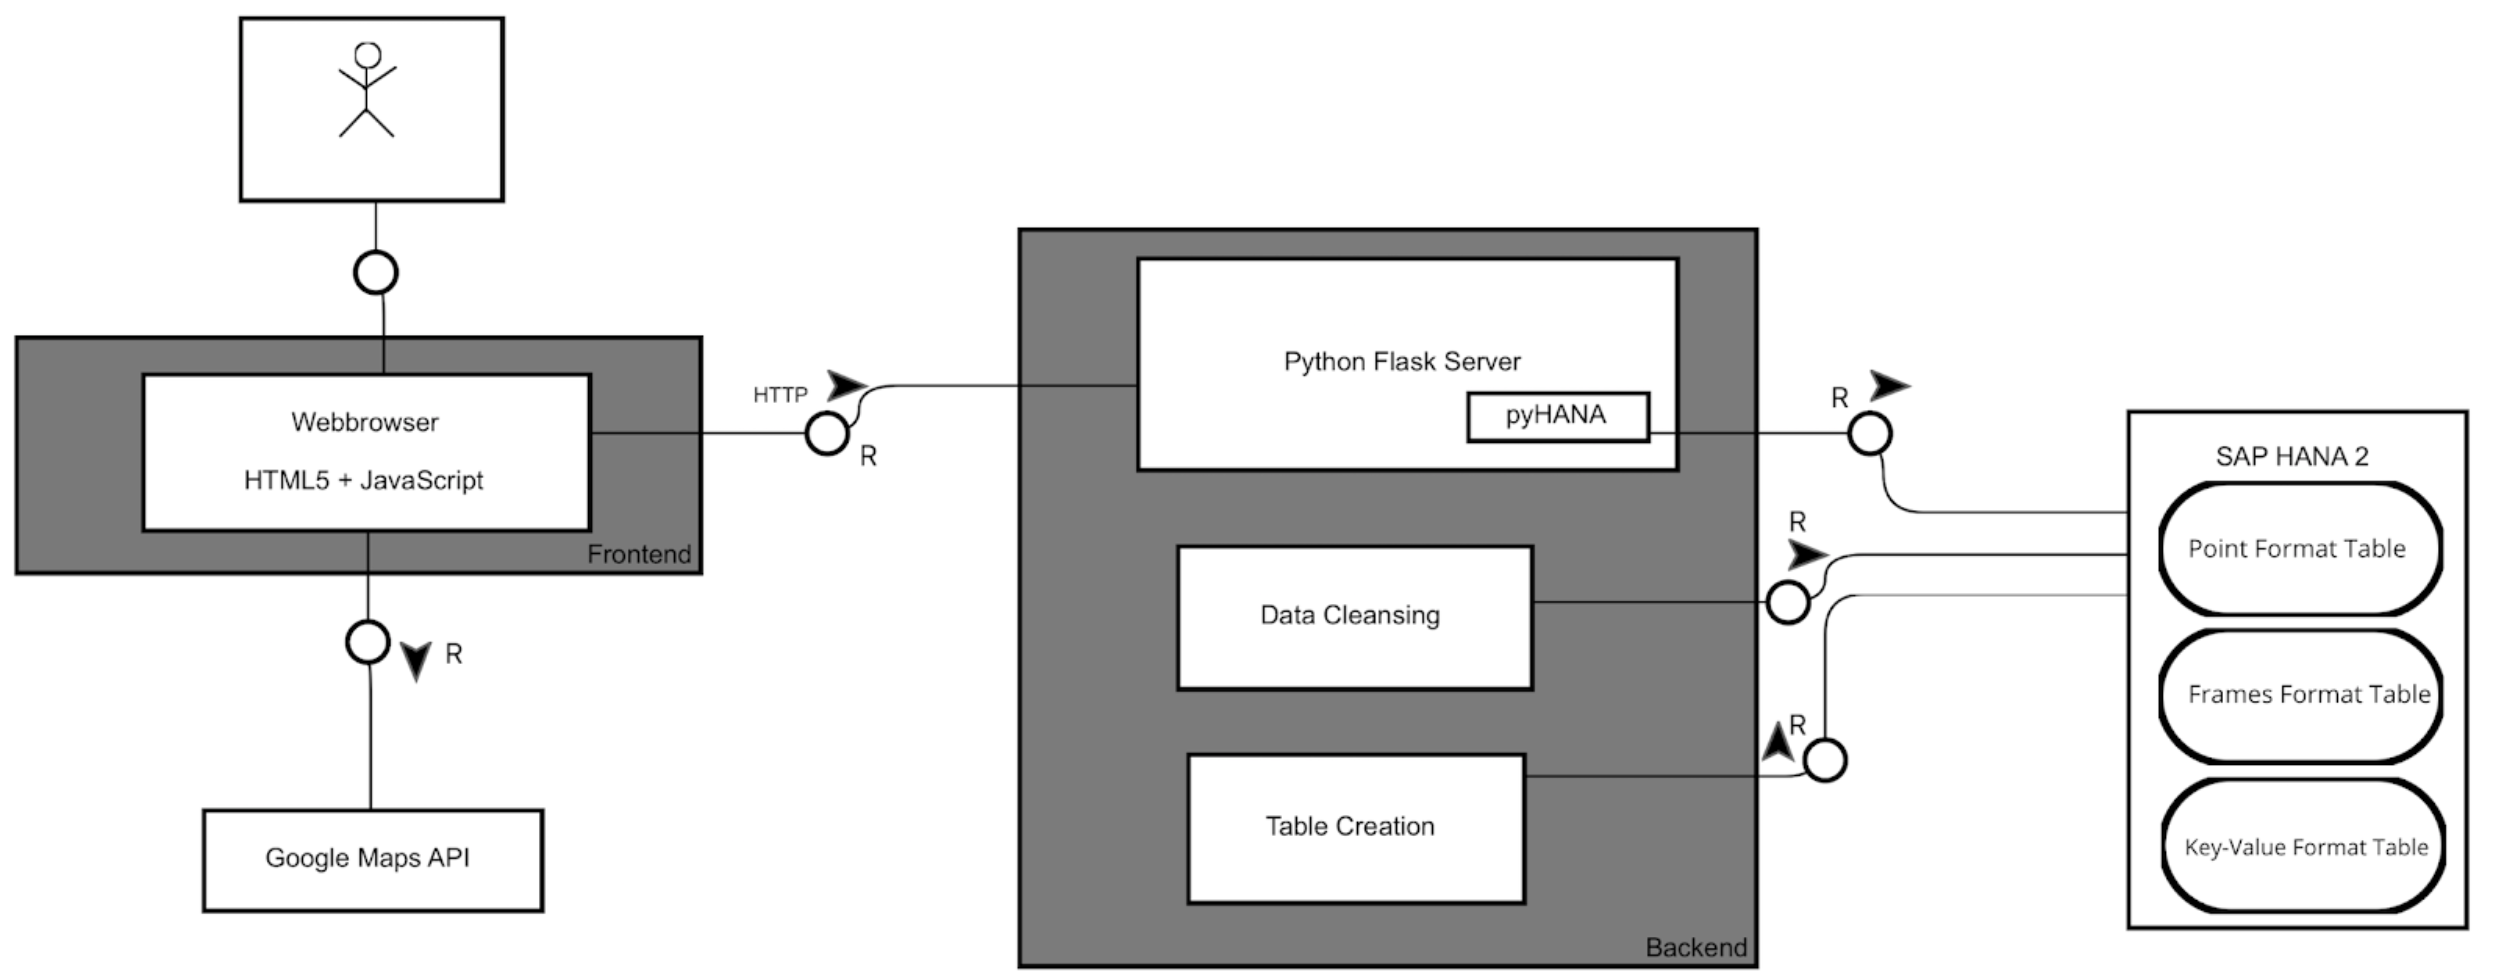
\includegraphics[width=0.8\textwidth]{img/architecture.png}
\caption{System architecture}
\label{fig:architecture}
\end{figure*}

The backend essentially has a REST API which is written in Python and uses the Flask framework. It serves the static HTML and Javascript files, as well as redirecting requests to the database. The backend also has a few python scripts that are used to create tables and for the data cleansing.

The database, which we are using, is SAP HANA. It stores all of the data in different table formats. The table formats are elaborated in section \ref{sec:data_layouts}. The database has some procedures that can be executed to answer non trivial data requests (e.g. to get the calculated profits). 

The communication between the backend and the database in managed via pyHANA\footnote{\href{https://github.com/hpi-epic/pyHANA}{https://github.com/hpi-epic/pyHANA}}. pyHANA is a Python client for SAP HANA.


\subsection{Data Layouts}
\label{sec:data_layouts}

\subsection{Optimizations}

\section{Benchmark Results}

\section{Future Work}

% mehr daten hinzufuegen. kein problem, da alle queries optimiert wurden 

\section{Conclusion}

\section{References}

\end{document}
